\documentclass[11pt,a4paper,twoside]{article}%
\usepackage{amsmath}
\usepackage{amsfonts}
\usepackage{amssymb}
\usepackage{graphicx}%
\setcounter{MaxMatrixCols}{30}
%TCIDATA{OutputFilter=latex2.dll}
%TCIDATA{Version=5.50.0.2953}
%TCIDATA{CSTFile=40 LaTeX article.cst}
%TCIDATA{Created=Thursday, December 26, 2013 11:29:10}
%TCIDATA{LastRevised=Monday, August 10, 2015 11:24:19}
%TCIDATA{<META NAME="GraphicsSave" CONTENT="32">}
%TCIDATA{<META NAME="SaveForMode" CONTENT="1">}
%TCIDATA{BibliographyScheme=Manual}
%TCIDATA{<META NAME="DocumentShell" CONTENT="Standard LaTeX\Blank - Standard LaTeX Article">}
%BeginMSIPreambleData
\providecommand{\U}[1]{\protect\rule{.1in}{.1in}}
%EndMSIPreambleData
\newtheorem{theorem}{Theorem}
\newtheorem{acknowledgement}[theorem]{Acknowledgement}
\newtheorem{algorithm}[theorem]{Algorithm}
\newtheorem{axiom}[theorem]{Axiom}
\newtheorem{case}[theorem]{Case}
\newtheorem{claim}[theorem]{Claim}
\newtheorem{conclusion}[theorem]{Conclusion}
\newtheorem{condition}[theorem]{Condition}
\newtheorem{conjecture}[theorem]{Conjecture}
\newtheorem{corollary}[theorem]{Corollary}
\newtheorem{criterion}[theorem]{Criterion}
\newtheorem{definition}[theorem]{Definition}
\newtheorem{example}[theorem]{Example}
\newtheorem{exercise}[theorem]{Exercise}
\newtheorem{lemma}[theorem]{Lemma}
\newtheorem{notation}[theorem]{Notation}
\newtheorem{problem}[theorem]{Problem}
\newtheorem{proposition}[theorem]{Proposition}
\newtheorem{remark}[theorem]{Remark}
\newtheorem{solution}[theorem]{Solution}
\newtheorem{summary}[theorem]{Summary}
\newenvironment{proof}[1][Proof]{\noindent\textbf{#1.} }{\ \rule{0.5em}{0.5em}}
\topmargin -0.7in
\oddsidemargin -0.30in
\evensidemargin -0.7in
\textwidth 7.3in
\textheight 9.5in
\begin{document}

\begin{center}
\textbf{\textsf{Estad\'{\i}stica (Qu\'{\i}mica) - Primer Cuatrimestre - 2020 - Coronavirus}}\\

\textbf{Pr\'{a}ctica 4 - Estad\'{\i}stica Descriptiva\vspace{-0.1in}}
\end{center}

\begin{enumerate}
\item Una muestra est\'{a}ndar de suero sangu\'{\i}neo contiene $42.0$ g de
alb\'{u}mina por litro. Cuatro laboratorios (A -- D) realizan seis
determinaciones cada uno (en el mismo d\'{\i}a) de la concentraci\'{o}n de
alb\'{u}mina, con los siguientes resultados (en g/l):%
\[%
\begin{tabular}
[c]{|c|}\hline
A\qquad42.5\qquad41.6\qquad42.1\qquad41.9\qquad41.1\qquad42.2\\
B\qquad39.8\qquad43.6\qquad42.1\qquad40.1\qquad43.9\qquad41.9\\
C\qquad43.5\qquad42.8\qquad43.8\qquad43.1\qquad42.7\qquad43.3\\
D\qquad39.4\qquad41.9\qquad40.7\qquad40.3\qquad42.6\qquad39.0\\\hline
\end{tabular}
\ \
\]
(para resolver este ejercicio, mire las instrucciones en el archivo
\texttt{instruccionesej1.R} cuyo link figura cerquita de d\'{o}nde baj\'{o}
este archivo).

\begin{enumerate}
\item Grafique en cada caso los datos en un Diagrama de Punto, todos en la
misma escala.

\item Comente la insesgadez (o exactitud) y la precisi\'{o}n de cada una de
estas series de resultados. \textquestiondown Qu\'{e} estad\'{\i}sticos
utiliz\'{o} para responder?
\end{enumerate}

\item[2.] En un experimento se midi\'{o} la temperatura de sublimaci\'{o}n del
iridio y del rodio. Los datos figuran m\'{a}s adelante. La siguiente
instrucci\'{o}n puede ser \'{u}til para leer el archivo en R (ya que las
longitudes de los dos conjuntos de datos son diferentes).%
\[
\text{\texttt{read.table(file.choose(),head=TRUE,fill=TRUE)}}%
\]


\begin{enumerate}
\item Compare los dos conjuntos de datos mediante histogramas y box plots.
Grafique los dos boxplots en el mismo gr\'{a}fico.

\item Halle las medias, las medianas y las medias podadas al 10\% y 20\%. Compare.

\item Halle el desv\'{\i}o est\'{a}ndar, la distancia intercuartil y la MAD
como medidas de dispersi\'{o}n.

\item Halle los percentiles 0.90, 0.75, 0.50, 0.25 y 0.10.

\item Se cuenta con la siguiente informaci\'{o}n adicional sobre este conjunto
de datos: se listaron en el orden en que fueron tomadas. Grafique las
observaciones en el orden en que fueron tomadas.\textquestiondown Es razonable
el modelo de errores independientes e id\'{e}nticamente distribuidos?
\textquestiondown Ser\'{\i}a correcto analizar todo el conjunto de datos?
\textquestiondown A partir de cu\'{a}l observaci\'{o}n considera que el
proceso se ha estabilizado?

\item Sobre el conjunto de datos correspondiente al proceso estabilizado,
resuelva nuevamente los \'{\i}tems a) -- d).%
\[%
\begin{tabular}
[c]{|c|}\hline
IRIDIO\\\hline
136.6\qquad145.2\qquad151.5\qquad162.7\qquad159.1\qquad159.8\qquad
160.8\qquad173.9\qquad160.1\\
160.4\qquad161.1\qquad160.6\qquad160.2\qquad159.5\qquad160.3\qquad
159.2\qquad159.3\qquad159.6\\
160.0\qquad160.2\qquad160.1\qquad160.0\qquad159.7\qquad159.5\qquad
159.5\qquad159.6\qquad159.5\\\hline
\end{tabular}
\ \
\]%
\[%
\begin{tabular}
[c]{|c|}\hline
RODIO\\\hline
126.4\qquad135.7\qquad132.9\qquad131.5\qquad131.1\qquad131.1\qquad
131.9\qquad132.7\\
133.3\qquad132.5\qquad133.0\qquad133.0\qquad132.4\qquad131.6\qquad
132.6\qquad132.2\\
131.3\qquad131.2\qquad132.1\qquad131.1\qquad131.4\qquad131.2\qquad
131.1\qquad131.1\\\hline
\end{tabular}
\ \
\]

\end{enumerate}

\item[3.] En un estudio nutricional se consideran las calor\'{\i}as y el
contenido de sodio de tres tipos de salchichas y se obtuvieron los datos que
se muestran en la tabla final.

\begin{enumerate}
\item Realice un histograma para las calor\'{\i}as de cada tipo de salchichas.
\textquestiondown Observa grupos en alg\'{u}n gr\'{a}fico?
\textquestiondown Cu\'{a}ntos grupos observa? \textquestiondown Observa
alg\'{u}n candidato a outlier?

\item Repita con la cantidad de sodio.

\item Realice los box plots paralelos para las calor\'{\i}as.
\textquestiondown Observa la misma cantidad de grupos que antes?
\textquestiondown A qu\'{e} conclusi\'{o}n llega? De acuerdo con los box plots
hallados, \textquestiondown c\'{o}mo caracterizar\'{\i}a la diferencia entre
los tres tipos de salchichas desde el punto de vista de las calor\'{\i}as?

\item \textquestiondown Le parece que los datos sustentan la igualdad del
contenido medio cal\'{o}rico de las tres variedades?%
\[%
\begin{tabular}
[c]{|c|c|cc|c|c|}\hline
\multicolumn{2}{|c|}{A} & \multicolumn{2}{|c|}{B} & \multicolumn{2}{|c|}{C}%
\\\hline
Calor\'{\i}as & Sodio & Calor\'{\i}as & Sodio & Calor\'{\i}as & Sodio\\\hline
186 & 495 & 173 & 458 & 129 & 430\\
181 & 477 & 191 & 506 & 132 & 375\\
176 & 425 & 182 & 473 & 102 & 396\\
149 & 322 & 190 & 545 & 106 & 383\\
184 & 482 & 172 & 496 & 94 & 387\\
190 & 587 & 147 & 360 & 102 & 442\\
158 & 370 & 146 & 387 & 87 & 359\\
139 & 322 & 139 & 386 & 99 & 357\\
175 & 479 & 175 & 507 & 170 & 528\\
148 & 375 & 136 & 393 & 113 & 513\\
152 & 330 & 179 & 405 & 135 & 426\\
111 & 300 & 153 & 372 & 142 & 513\\
141 & 386 & 107 & 144 & 86 & 358\\
153 & 401 & 195 & 511 & 143 & 581\\
190 & 645 & 135 & 405 & 152 & 588\\
157 & 440 & 140 & 428 & 146 & 522\\
131 & 317 & 138 & 339 & 144 & 545\\
149 & 319 &  &  &  & \\
135 & 298 &  &  &  & \\
132 & 253 &  &  &  & \\\hline
\end{tabular}
\ \
\]

\end{enumerate}

\item[4.] Los siguientes datos corresponden a 100 determinaciones repetidas de
la concentraci\'{o}n de ion nitrato (en $\mu$g/l), 50 de ellas corresponden a
un grupo de estudiantes (Grupo A) y las restantes 50 a otro grupo (Grupo B):%
\[%
\begin{tabular}
[c]{|cccc|cccc|}\hline
\multicolumn{4}{|c|}{Grupo A} & \multicolumn{4}{|c|}{Grupo B}\\\hline
0.51 & 0.51 & 0.50 & 0.50 & 0.61 & 0.67 & 0.70 & 0.56\\
0.51 & 0.50 & 0.48 & 0.50 & 0.61 & 0.67 & 0.63 & 0.75\\
0.49 & 0.50 & 0.47 & 0.50 & 0.55 & 0.49 & 0.75 & 0.55\\
0.51 & 0.48 & 0.52 & 0.49 & 0.65 & 0.77 & 0.64 & 0.58\\
0.51 & 0.49 & 0.52 & 0.51 & 0.73 & 0.51 & 0.66 & 0.65\\
0.51 & 0.48 & 0.52 & 0.49 & 0.65 & 0.57 & 0.61 & 0.53\\
0.52 & 0.53 & 0.49 & 0.51 & 0.53 & 0.64 & 0.52 & 0.69\\
0.48 & 0.51 & 0.50 & 0.47 & 0.54 & 0.57 & 0.63 & 0.62\\
0.51 & 0.49 & 0.50 & 0.50 & 0.68 & 0.56 & 0.58 & 0.58\\
0.50 & 0.49 & 0.53 & 0.47 & 0.59 & 0.62 & 0.60 & 0.66\\
0.51 & 0.50 & 0.49 & 0.48 & 0.61 & 0.54 & 0.63 & 0.61\\
0.53 & 0.52 & 0.51 & 0.51 & 0.69 & 0.63 & 0.53 & 0.48\\
0.46 & 0.49 &  &  & 0.65 & 0.61 &  & \\\hline
\end{tabular}
\
\]


\begin{enumerate}
\item Estudie si la distribuci\'{o}n de los conjuntos de datos para ambos
grupos es normal, realizando los correspondientes histogramas y superponiendo
la curva normal. Adem\'{a}s dibuje los qqplots para cada conjunto de datos.

\item \textquestiondown Le parece a partir de estos datos que ambos grupos
est\'{a}n midiendo lo mismo? Responda comparando medidas de centralidad y de
dispersi\'{o}n de los datos. Hacer un box-plot de ambos conjuntos de datos en
el mismo gr\'{a}fico.
\end{enumerate}

\item[5.] En una clase grande, hay 150 estudiantes hombres y 100 mujeres, los
estudiantes promediaban en altura 178cm, con un desv\'{\i}o standard de 25cm y
las estudiantes promediaban 162cm, con un desv\'{\i}o standard de 25cm.
Tomando conjuntamente los hombres y las mujeres:

\begin{enumerate}
\item La altura promedio es \_\_\_\_\_\_\_\_\_\_\_\_\_\_\_\_\_\_\_\_\_\_.

\item El desv\'{\i}o est\'{a}ndar de las alturas es \textquestiondown un poco
mayor que 25cm, exactamente 25cm, \'{o} un poco inferior a 25cm?
\end{enumerate}

\item[6.] Con la finalidad de incrementar las lluvias en zonas des\'{e}rticas,
se desarroll\'{o} un m\'{e}todo que consiste en el bombardeo de la nube con
\'{a}tomos. Para evaluar la efectividad del m\'{e}todo se realiz\'{o} el
siguiente experimento:

\begin{itemize}
\item Para cada nube que se pod\'{\i}a bombardear se decidi\'{o} al azar si se
la trataba o no.

\item Las nubes no tratadas fueron denominadas nubes controles.
\end{itemize}

Las tablas presentan la cantidad de agua ca\'{\i}da de 26 nubes tratadas y 26
nubes controles.%
\[%
\begin{tabular}
[c]{|c|}\hline
NUBES TRATADAS\\\hline
129.6\qquad31.4\qquad2745.6\qquad489.1\qquad430.0\qquad302.8\qquad
119.0\qquad4.1\qquad92.4\\
17.5\qquad200.7\qquad274.7\qquad274.7\qquad7.7\qquad1656.0\qquad
978.0\qquad198.6\qquad703.4\\
1697.8\qquad334.1\qquad118.3\qquad255.0\qquad115.3\qquad242.5\qquad
32.7\qquad40.6\\\hline
\end{tabular}
\
\]%
\[%
\begin{tabular}
[c]{|c|}\hline
NUBES CONTROLES\\\hline
26.1\qquad26.3\qquad87.0\qquad95.0\qquad372.4\qquad0.01\qquad17.3\qquad
24.4\qquad11.5\\
321.2\qquad68.5\qquad81.5\qquad47.3\qquad28.6\qquad830.1\qquad345.5\qquad
1202.6\qquad36.6\\
4.9\qquad4.9\qquad41.1\qquad29.9\qquad163.0\qquad244.3\qquad147.8\qquad
21.7\\\hline
\end{tabular}
\
\]


\begin{enumerate}
\item Realice box plots para ambos grupos. \textquestiondown Le parece que el
m\'{e}todo produce alg\'{u}n efecto?

\item Analice la normalidad realizando\ qqplots e histogramas (de densidad)
para ambos conjuntos de datos y superponiendo la curva normal. Para hacerlo,
considere la instrucci\'{o}n (donde en el vector \texttt{ww} guardamos los
datos de controles o tratadas):%
\begin{align*}
\text{\texttt{hist(ww,probability}} &  \text{\texttt{=T)}}\\
\text{\texttt{equis}} &  \text{\texttt{%
%TCIMACRO{\TEXTsymbol{<}}%
%BeginExpansion
$<$%
%EndExpansion
-seq(min(ww),max(ww),by=0.01)}}\\
\text{\texttt{lines(equis,dnorm(equis,\ mean\ }} &
\text{\texttt{=\ mean(ww),sd\ =\ sqrt(var(ww))),col=2,lwd=2)}}%
\end{align*}


\item Realice la transformaci\'{o}n log a los datos y repita b) para los datos transformados.
\end{enumerate}

\item[7.] El histograma muestra la distribuci\'{o}n de presi\'{o}n
sangu\'{\i}nea de 15000 mujeres en estudio. Utilice el histograma para
responder las siguientes preguntas:%

%TCIMACRO{\FRAME{fhF}{3.3261in}{2.5521in}{0pt}{}{}{histogramadescriptiva.jpg}%
%{\special{ language "Scientific Word";  type "GRAPHIC";
%maintain-aspect-ratio TRUE;  display "USEDEF";  valid_file "F";
%width 3.3261in;  height 2.5521in;  depth 0pt;  original-width 3.2811in;
%original-height 2.5105in;  cropleft "0";  croptop "1";  cropright "1";
%cropbottom "0";
%filename 'histogramadescriptiva.JPG';file-properties "XNPEU";}}}%
%BeginExpansion
\begin{figure}
[ht]
\begin{center}
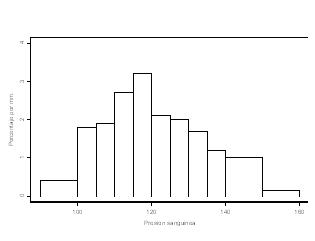
\includegraphics[width=0.75\textwidth]
{histogramadescriptiva.jpg}%
\end{center}
\end{figure}
%EndExpansion


\begin{enumerate}
\item \textquestiondown El porcentaje de mujeres con presi\'{o}n superior a
los 130mm es m\'{a}s cercano a 25\%, 50\% o 75\%?

\item \textquestiondown El porcentaje de mujeres con presi\'{o}n entre 90 y
160mm es m\'{a}s cercano al 1\%, 50\% o 99\%?

\item \textquestiondown Cu\'{a}l intervalo tiene m\'{a}s mujeres: 130-140mm o 140-150mm?

\item \textquestiondown Cu\'{a}l intervalo tiene m\'{a}s mujeres: 130-135mm o 140-150mm?

\item En el intervalo 125-130mm la altura del histograma es de alrededor de
2.2\% por mm. \textquestiondown Qu\'{e} porcentaje de mujeres tuvo presi\'{o}n
en ese intervalo?
\end{enumerate}

\item[8.] Considere $x_{1},\ldots,x_{n}$ una muestra de una poblaci\'{o}n
cualquiera. Sean $\overline{x}$ y $\widetilde{x}$\ la media y la mediana
muestral respectivamente.

\begin{enumerate}
\item Si se suma una constante $a$ a cada uno de los $x_{i}$ de la muestra,
obteni\'{e}ndose $y_{i}=x_{i}+a$, \textquestiondown c\'{o}mo se relacionan
$\overline{x}$ con $\overline{y}$ y $\widetilde{x}$ con $\widetilde{y}$?

\item Si cada uno de los $x_{i}$ es multiplicado por una constante $b$,
obteni\'{e}ndose $y_{i}=bx_{i}$, \textquestiondown c\'{o}mo se relacionan
$\overline{x}$ con $\overline{y}$ y $\widetilde{x}$ con $\widetilde{y}$?
\end{enumerate}

\item[9.] Sea $s_{X}^{2}$ la varianza muestral correspondiente a los datos
$x_{1},\ldots,x_{n}$ observados. Demuestre que

\begin{enumerate}
\item $s_{X}^{2}=\frac{1}{n-1}\sum_{i=1}^{n}x_{i}^{2}-\frac{n}{n-1}%
\overline{x}^{2}$.

\item Probar que si $y_{i}=x_{i}+a$ con $a$\ constante, entonces $s_{X}=s_{Y}$.

\item Probar que si $y_{i}=bx_{i}$ con $b$\ constante, entonces $s_{X}%
=\left\vert b\right\vert s_{Y}$.
\end{enumerate}
\end{enumerate}


\end{document}
